\paragraph{QuizziPedia::Back-End::App::Routers::LangRouter}
\label{QuizziPedia::Back-End::App::Routers::LangRouter}
\begin{figure}[ht]
	\centering
	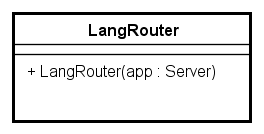
\includegraphics[scale=0.8]{UML/Classi/Back-End/QuizziPedia_Back-End_App_Routers_LangRouter.png}
	\caption{QuizziPedia::Back-End::App::Routers::LangRouter}
\end{figure}
\FloatBarrier
	\begin{itemize}
		\item \textbf{Descrizione}: classe che gestisce le richieste relative alla lingua;
		\item \textbf{Utilizzo}: viene utilizzata per chiamare il \textit{controller\ped{G}} che si occupa di cambiare la lingua dell'applicazione;
		\item \textbf{Relazioni con altre classi}:
			\begin{itemize}
				\item \textbf{IN \texttt{Server}}: classe che avvia il \textit{server\ped{G}}. Nello specifico apre una connessione al database tramite \textit{Mongoose\ped{G}}, invoca il \textit{middleware\ped{G}} \textit{Express\ped{G}} passando un riferimento al database \textit{MongoDB\ped{G}} come parametro in modo che possa configurarsi con esso, invoca il \textit{middleware\ped{G}} \textit{Passport\ped{G}} ed infine si mette in ascolto su una determinata porta; è il componente \textit{client\ped{G}} del pattern \textit{Chain of responsability\ped{G}}. Utilizza i moduli \textit{Mongoose\ped{G}}, \textit{Express\ped{G}}, \textit{Passport\ped{G}};
				\item \textbf{OUT \texttt{NotFoundHandler}}: classe che si occupa della gestione dell'errore di una pagina non trovata. Componente \textit{ConcreteHandler\ped{G}} del \textit{design pattern\ped{G}} \textit{Chain-of-responsability\ped{G}};
				\item \textbf{OUT \texttt{LangController}}: classe che gestisce la logica applicativa riguardante il passaggio della traduzione delle variabili.
			\end{itemize}
		\item \textbf{Metodi}:
			\begin{itemize}
				\item \texttt{+ LangRouter(app: Server)} \\
				Contiene diverse \textit{ruote\ped{G}} che vengono configurate all'avvio del \textit{server\ped{G}}. Queste ultime ricevono le richieste del \textit{client\ped{G}} e passano il controllo al \textit{ConcreteHandler\ped{G}} successivo. \\
				\textbf{Parametri}:
					\begin{itemize}
						\item \texttt{app: Server} \\
						Rappresenta l'istanza del server su cui configurare i \textit{ruote\ped{G}} che mappano i\\ \textit{controllers\ped{G}} specifici.
					\end{itemize}
			\end{itemize}
	\end{itemize}